\documentclass[nobib,nofonts]{tufte-handout}

%\geometry{showframe} % display margins for debugging page layout

%%% MF additions
\usepackage[nographicx, nohyperref, nosubcaption, nogb4e, nobiblatex]{../99-auxiliary-files/00-mypackages}
\usepackage{../99-auxiliary-files/00-mycommands}
\usepackage{../99-auxiliary-files/00-myenvironments}

\usepackage{titlesec}
\usepackage{etoolbox}
\usepackage{tikz-qtree}
\usepackage{subcaption}

% \titleformat{\section}
% {\large\bfshape}{\thesection}{1em}{}

\setcounter{secnumdepth}{5}
\renewcommand\thesection{\arabic{section}}

% this length controls tha hanging indent for titles
% change the value according to your needs
\newlength\titleindent
\setlength\titleindent{0.7cm}

\pretocmd{\paragraph}{\stepcounter{subsection}}{}{}
\pretocmd{\subparagraph}{\stepcounter{subsubsection}}{}{}

\titleformat{\chapter}[block]
  {\normalfont\huge\bfseries}{}{0pt}{\hspace*{-\titleindent}}

\titleformat{\section}
  {\normalfont\Large\itshape}{\llap{\parbox{\titleindent}{\thesection\hfill}}}{0em}{}

\titleformat{\subsection}
  {\normalfont\itshape}{\llap{\parbox{\titleindent}{\thesubsection\hfill}}}{0em}{}

\titleformat{\subsubsection}
  {\normalfont\normalsize\itshape}{\llap{\parbox{\titleindent}{\thesubsubsection}}}{0em}{}

\titleformat{\paragraph}[runin]
  {\normalfont\normalsize\itshape}{}{-0.7cm}{}[\xspace \ \ \ \ ]

\titleformat{\subparagraph}[runin]
  {\normalfont\normalsize}{\llap{\parbox{\titleindent}{\thesubsubsection\hfill}}}{0em}{}

\titlespacing*{\chapter}{0pt}{0pt}{20pt}
\titlespacing*{\subsubsection}{0pt}{3.25ex plus 1ex minus .2ex}{1.5ex plus .2ex}
\titlespacing*{\paragraph}{0pt}{3.25ex plus 1ex minus .2ex}{0em}
\titlespacing*{\subparagraph}{0pt}{3.25ex plus 1ex minus .2ex}{0em}

\DefineNamedColor{named}{mygray2}{cmyk}{0.55,0.25,0.25,0.25}
\newcommand{\mygray}[1]{\textcolor{mygray2}{#1}}

%%% Tufte style
\usepackage{graphicx} % allow embedded images
  \setkeys{Gin}{width=\linewidth,totalheight=\textheight,keepaspectratio}
  \graphicspath{{graphics/}} % set of paths to search for images

\usepackage{fancyvrb} % extended verbatim environments
  \fvset{fontsize=\normalsize}% default font size for fancy-verbatim environments

% Standardize command font styles and environments
\newcommand{\doccmd}[1]{\texttt{\textbackslash#1}}% command name -- adds backslash automatically
\newcommand{\docopt}[1]{\ensuremath{\langle}\textrm{\textit{#1}}\ensuremath{\rangle}}% optional command argument
\newcommand{\docarg}[1]{\textrm{\textit{#1}}}% (required) command argument
\newcommand{\docenv}[1]{\textsf{#1}}% environment name
\newcommand{\docpkg}[1]{\texttt{#1}}% package name
\newcommand{\doccls}[1]{\texttt{#1}}% document class name
\newcommand{\docclsopt}[1]{\texttt{#1}}% document class option name
\newenvironment{docspec}{\begin{quote}\noindent}{\end{quote}}% command specification environment

\newcommand{\proplog}{\acro{PropLog}}

%%%%%%%%%%%%%%%%%%%%%%%%%%%%%%%%%%%%%%%%%%%%%%%%%%

% \usepackage[sc,osf]{mathpazo}
% \linespread{1.05}



\title{Propositional logic}

\author[M.~Franke]{Michael Franke}

\date{} % without \date command, current date is supplied

\begin{document}

\maketitle

\begin{abstract}
\noindent
Syntax \& semantics of propositional logic; truth-tables; tautologies vs.~contraditions vs.~contingencies; translations from natural language into propositional logic; argument schemas \& logical validity.
\end{abstract}

\section{The language of propositional logic}

Propositional logic (\proplog) studies how propositions are combined by logical operators, which closely correspond to certain sentential connectives in natural language (such as \emph{and}, \emph{or}, \emph{if}, or \emph{not}).
A \textit{proposition} in the sense of \proplog is a minimal unit of thought which can be evaluated as true or false independently of other propositions.\sidenote{The notion of a proposition in this sense is not unproblematic. For example, a case like ``\textit{This pixel is red.}'' seems like a minimal unit of truth-evaluable information about the color of a particular pixel, but it is not independent of another statement like ``\textit{This pixel is blue.}''. (Historically, this problem related to color was a problem brought up famously by Frank Ramsey in response to the early logical work of Ludwig Wittgenstein.)}
For example, the logical structure of the following sentence:
%
\begin{align*}
  \underbrace{\text{The earth is round }}_{p}
  \underbrace{\text{ and }}_{\wedge}
  \underbrace{\text{ the moon is made of cheese.}}_{q}
\end{align*}
%
could be analyzed as composed of two propositions, viz., the proposition denoted here with \emph{proposition letter} $p$ that the earth is round and the proposition denoted by $q$ that the moon is made of cheese.
These two propositions are connected by a logical operator ``and'', for which we write $\wedge$ in \proplog.
The logical structure of the complex sentence above can therefore be written as $p \wedge q$ in \proplog.

\subsection{Proposition letters \& sentential connectives}

The language of \proplog is formed by:
\begin{enumerate}[(i)]
  \item a set of \emph{proposition letters} $\mathfrak{P} = \set{p, q, r, s, p_{1}, q_{27}, \dots}$, and
  \item a set of \emph{sentential connectives} $\set{\neg, \wedge, \vee, \rightarrow, \leftrightarrow}$\sidenote{You will also find terminology like \emph{logical connectives} or \emph{logical operators}. There may be additional connectives used by some logicians or textbooks, and you might find slightly different symbols for the same notions in some places}
\end{enumerate}
The sentential connectives have names and are intended to correspond (approximately) to natural language paraphrases:\sidenote{The names and the (approximate) correspondence are earned by the \emph{semantics} which we will give to these symbols later on.}

\begin{center}
  \begin{tabular}{llc}
    name & paraphrase & symbol \\ \midrule
    negation     & ``not''   & $\neg$ \\
    conjunction  & ``and''   & $\wedge$ \\
    disjunction  & ``or''    & $\vee$ \\
    implication  & ``if \dots, then \dots''    & $\rightarrow$ \\
    equivalence  & ``if and only of''    & $\leftrightarrow$ \\
  \end{tabular}
\end{center}

\subsection{Formulas}

The language $\mathfrak{L}$ of \proplog is the set of all \emph{formulas} which are recursively defined as follows:\sidenote{We will make consistent use of Greek letters $\varphi, \psi, \chi, \dots$ as variables for formulas.}
\begin{enumerate}[(i)]
  \item Every proposition letter is a formula.
  \item If $\varphi$ is a formula, so is $\neg \varphi$.
  \item If $\varphi$ and $\psi$ are formulas, so are:
        \vspace*{-0.4cm}
        \begin{multicols}{4}
          \begin{enumerate}[a.]
            \item ($\varphi \wedge \psi$)
            \item ($\varphi \vee \psi$)
            \item ($\varphi \rightarrow \psi$)
            \item ($\varphi \leftrightarrow \psi$)
          \end{enumerate}
        \end{multicols}
        \vspace*{-0.4cm}
  \item Anything that cannot be constructed by (i)--(iii) is not a formula.
\end{enumerate}
Examples for formulas of \proplog are:\sidenote{We conventionally omit the outermost parentheses of a formula.}
\begin{align*}
  p & p \wedge p \\
  p \rightarrow \neg q & (p \vee q) \leftrightarrow r
\end{align*}
Examples of strings made of proposition letters and logical connectives which are \emph{not} formulas of \proplog are:
\begin{align*}
  (p) && \neg pq \\
  p \neg \rightarrow \neg q && p \vee q \leftrightarrow r
\end{align*}

\subsection{Syntactic trees}

The recursive definition for formulas of \proplog gives an internal structure to each formula.
Take the example $p \wedge \neg q$.
There is only one way in which this formulas could have been generated by a constructive process that follows the recursive definition above.
In the last step of that process, the two subformulas $\varphi = p$ and $\psi = \neg q$ have been combined to form an expression of the form $\varphi \wedge \psi$ using the rule (iii) part a.
The first subformula  $\varphi = p$ is constructed by rule (i).
The second formula can only be constructed by first using rule (i) to introduce $q$ and then using rule (ii) to introduce the negation sign.

A \emph{syntactic tree} is a useful visual illustration of the internal structure of a formula.
The syntactic tree of formula $p \wedge \neg q$ is this:

\begin{center}
  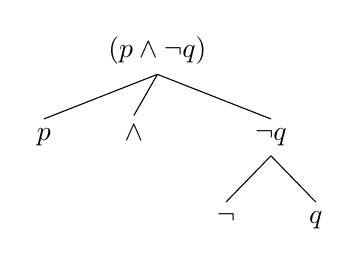
\begin{tikzpicture}[sibling distance=20pt, level distance=30pt]
    \Tree [.{$(p \wedge \neg q)$} [. $p$ ] [. $\wedge$ ] [.{$\neg q$} [. $\neg$ ] [. $q$ ] ]  ]
  \end{tikzpicture}
\end{center}

The construction of a complex formula, and therefore its syntactic tree, is always recoverable by following the introduction of the parentheses in step (iii).
This is illustrated by the minimal pair in Figure~\ref{fig:syntactic-trees}.

\begin{figure}
  \centering

  \begin{subfigure}[b]{0.45\textwidth}
    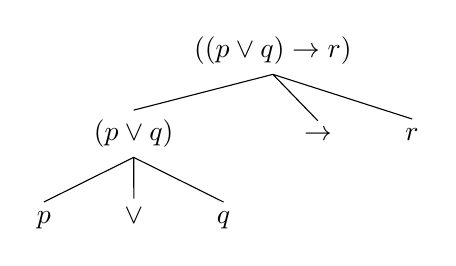
\begin{tikzpicture}[sibling distance=20pt, level distance=30pt]
      \Tree [.{$((p \vee q) \rightarrow r)$} [.{$(p \vee q)$} [. {$p$} ] [. {$\vee$} ] [. {$q$} ] ]  [. $\rightarrow$ ] [. $r$ ] ]
    \end{tikzpicture}
    \caption{Tree for $((p \vee q) \rightarrow r)$}
  \end{subfigure}
  \hfill
  \begin{subfigure}[b]{0.45\textwidth}
    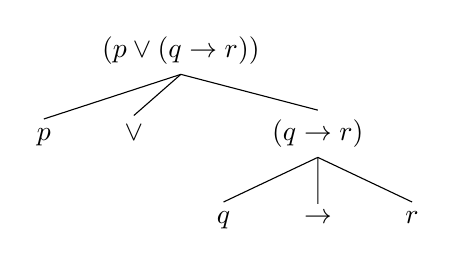
\begin{tikzpicture}[sibling distance=20pt, level distance=30pt]
      \Tree [.{$(p \vee (q \rightarrow r))$} [. $p$ ] [. $\vee$ ] [.{$(q \rightarrow r)$} [. {$q$} ] [. {$\rightarrow$} ] [. {$r$} ] ] ]
    \end{tikzpicture}
    \caption{Tree for $(p \vee (q \rightarrow r))$}
  \end{subfigure}

  \caption{Examples of syntactic trees}
  \label{fig:syntactic-trees}
\end{figure}

\subsection{Atomic \& complex formulas}

A formula of \proplog which consist of a single proposition letter is also called \emph{atomic formula.}
Any formula of \proplog which is not atomic is also called a \emph{complex formula}.
Each complex formula has a \emph{main connective}.
The main connective is the last sentential connector introduced during the construction of the formula.
A complex formula is also often called by the name of its main connective.
For example, the formula $p \wedge \neg q$ has a conjunction as its main operator and could therefore be called a conjunction.
The formula $(p \vee q) \rightarrow r$ from Figure~\ref{fig:syntactic-trees}(a) is an implication, while the formula $p \vee (q \rightarrow r)$ from Figure~\ref{fig:syntactic-trees}(b) is a disjunction.

\bigskip
\noindent \colorbox{mygray}{\centering
  \begin{minipage}{1.0\textwidth}

    \begin{exercise}
      Determine which of the following strings are formulas of propositional logic. For any formula, determine its main operator.
      \begin{multicols}{2}
        \begin{enumerate}[a.]
          \item $q_{12}$
          \item $p, q \wedge r$
          \item $(p) \wedge q$
          \item $p \rightarrow (p \wedge p)$
          \item $(p \rightarrow) (p \wedge p)$
          \item $(p \vee \neg q) \leftrightarrow (r \rightarrow (\neg (p \vee \neg p)))$
        \end{enumerate}
      \end{multicols}
    \end{exercise}

    \begin{exercise}
      Draw the syntactic tree for each of the following formulas.
      \begin{multicols}{2}
        \begin{enumerate}[a.]
          \item $p \leftrightarrow q$
          \item $\neg p \wedge p$
          \item $p \rightarrow \neg (q \wedge r)$
          \item $(\neg p \vee \neg q) \wedge (r \rightarrow p )$
        \end{enumerate}
      \end{multicols}
    \end{exercise}
  \end{minipage}
}

\end{document}
